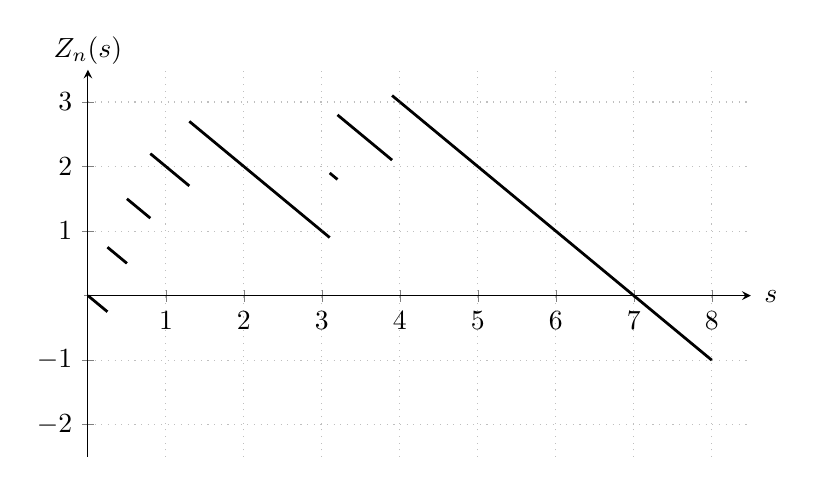
\begin{tikzpicture}

\begin{axis}[
axis x line=bottom,
axis y line=left,
grid = minor,
minor grid style={dotted},
xmin=0,
axis lines = middle,
xmax=8.5,
ymax = 3.5,
ymin  = -2.5,
xlabel={$s$},
x label style = {at={(axis description cs:1.055,0.415)},anchor=east},
ylabel={$Z_n(s)$},
y label style = {at={(axis description cs:0,1.11)},anchor=north},
xtick={1,...,8},
minor xtick = {1,...,8},
ytick={-2,...,3},
minor ytick={-2,...,3},
width = 10cm,
height = 6.5cm
]

%\addplot [
%line width=1.0pt
%]
%coordinates{
%	(0,0) (0.25,-0.25) (0.25,0.75) (0.5,0.5) (0.5,1.5) (0.8,1.2) (0.8,2.2) (1,2)
%	(1.3, 1.7) (1.3, 2.7) (2,2)
%	(3,1)
%	(3.1, 0.9) (3.1,1.9) (3.2,1.8) (3.2,2.8) (3.9,2.1) (3.9,3.1) (4,3)
%	(5,2) (6,1) (7,0) (8,-1)
%};

\addplot [line width=1.0pt]coordinates{(0,0) (0.25,-0.25)};
\addplot [line width=1.0pt]coordinates{(0.25,0.75) (0.5,0.5)};
\addplot [line width=1.0pt]coordinates{(0.5,1.5) (0.8,1.2)};
\addplot [line width=1.0pt]coordinates{(0.8,2.2) (1,2)};
\addplot [line width=1.0pt]coordinates{(1,2) (1.3, 1.7)};
\addplot [line width=1.0pt]coordinates{(1.3, 2.7) (2,2)};
\addplot [line width=1.0pt]coordinates{};
\addplot [line width=1.0pt]coordinates{(2,2) (3,1)};
\addplot [line width=1.0pt]coordinates{(3,1) (3.1, 0.9)};
\addplot [line width=1.0pt]coordinates{(3.1,1.9) (3.2,1.8)};
\addplot [line width=1.0pt]coordinates{(3.2,2.8) (3.9,2.1)};
\addplot [line width=1.0pt]coordinates{(3.9,3.1) (4,3)};
\addplot [line width=1.0pt]coordinates{(4,3) (8,-1)};

%% Dashed lines indicate end of vertex, but the xick already do that
%\addplot [dashed] coordinates {(1, -2.5) (1, 3.5)};
%\addplot [dashed] coordinates {(2, -2.5) (2, 3.5)};
%\addplot [dashed] coordinates {(3, -2.5) (3, 3.5)};
%\addplot [dashed] coordinates {(4, -2.5) (4, 3.5)};
%\addplot [dashed] coordinates {(5, -2.5) (5, 3.5)};
%\addplot [dashed] coordinates {(6, -2.5) (6, 3.5)};
%\addplot [dashed] coordinates {(7, -2.5) (7, 3.5)};
%\addplot [dashed] coordinates {(8, -2.5) (8, 3.5)};

\end{axis}

\end{tikzpicture} 